\chapter{Исследовательская часть}

\section{Замеры времени работы}

Для замеров времени работы функции запускались 10000 раз, на каждой итерации генерировались 2 квадратные матрицы, состоящие из случайных целых чисел в диапазоне от 0 до 1023. Результаты измерений суммировались, после чего выводилось среднее значение. Время работы было замерено с помощью функции $clock\_gettime()$ со значением первого параметра $CLOCK\_PROCESS\_CPUTIME\_ID$ \cite{clockgettime}. Все замеры проводились на ноутбуке Acer Swift 3x, процессор 11th Gen Intel(R) Core(TM) i7-1165G7 @ 2.80ГГц. 

Замеры при лучшем случае для алгоритма Винограда (чётное значение n) проводились для матриц размерами 50, 100, 150, 200, 250 строк и столбцов. Результаты представлены на рисунке \ref{fig:res1}.

\begin{figure}[h!]
	\centering
	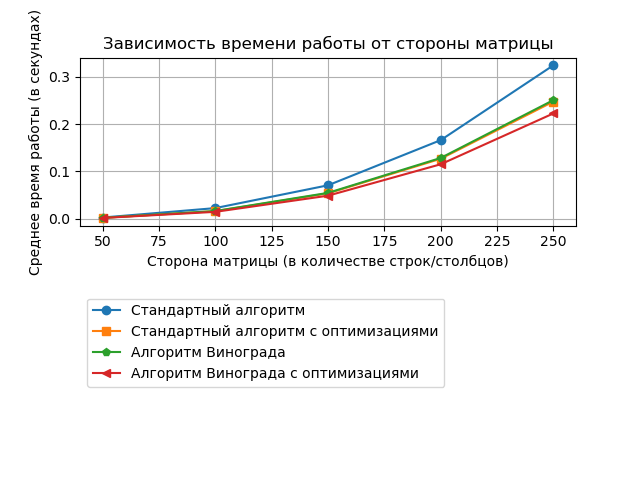
\includegraphics[width=0.8\textwidth]{tex_parts/graphicBest.png}
	\caption{\label{fig:res1} Результаты замера времени работы разных алгоритмов (лучший случай)}
\end{figure}

Результаты не совпали с оценкой ресурсной эффективности, так как реализации алгоритма Винограда оказались быстрее стандартных. Вероятно, это связано с тем, что умножение куда более трудоёмкая операция, чем было принято в модели вычислений.

Замеры при худшем случае для алгоритма Винограда (нечётное значение n) проводились для матриц размерами 51, 101, 151, 201, 251 строк и столбцов. Результаты представлены на рисунке \ref{fig:res2}
\begin{figure}[h!]
	\centering
	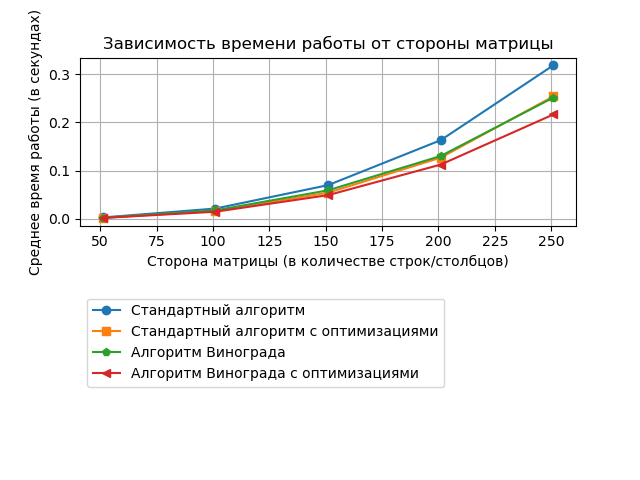
\includegraphics[width=0.8\textwidth]{tex_parts/graphicWorst.png}
	\caption{\label{fig:res2} Результаты замера времени работы разных алгоритмов (худший случай)}
\end{figure}

Результаты аналогичны лучшему случаю.

\section{Вывод}

В данном разделе были проведены замеры времени. Самой эффективной оказалась реализация алгоритма Винограда с оптимизациями, наименее эффективной - реализация стандартного алгоритма без оптимизаций. 
